\section{Method}
\label{sec:approach}
% \begin{itemize}
%     \item Inputs-outputs
%     \item Workflow + diagrams
%     \item Heuristics:
%     \begin{itemize}
%         \item Keyword extraction, more detailed than poster
%         \item Vector-based methods, more detailed than poster
%     \end{itemize}
%     \item Implementation:
%     \item \begin{itemize}
%         \item Trace graph + visuals
%         \item Dashboard
%         \item (Using same example for trace finding and trace graph)
%     \end{itemize}
% \end{itemize}

This section details our approach for discovering trace links in a software repository. Our approach takes a software repository and requirements as input and extract trace links between requirements and the software issues, commits, pull requests (PRs) by analyzing the textual fields of these artifacts. Our prototype tool visualizes the trace links and other information on the repository. Fig.~\ref{fig:sys-flow} presents the main steps of our approach.

\begin{figure}[htb]
    \centering
    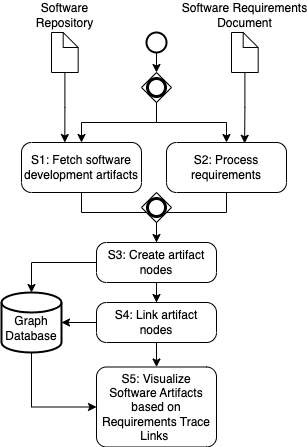
\includegraphics[width=0.65\linewidth]{figs/approach.png}
    \caption{Steps of our approach}
    \label{fig:sys-flow}
  \end{figure}

  The first two steps, \textsf{S1} and \textsf{S2}, concerns processing the two inputs of our approach, a software repository and natural language requirements, respectively. \textsf{S1} fetches issues, pull requests, and commits from a repository whose URL is given. Our prototype expects a Github repository, however our approach is general and can be applied to other repositories where the aforementioned development artifacts are present. Table~\ref{tab:artifactfeatures} presents the attributes of these artifacts that are used in our approach. Our prototype expects a text file containing requirements. It do not enforce a specific for requirements and is able to process the requirements that written in a hierarchical structure, which is a common practice.

        \begin{table}
        \centering
        \caption{Attributes of software development artifacts used in our approach}
        \label{tab:artifactfeatures}
        \begin{tabular}{lllll}
          \toprule
          & Requirement & Issue & PR & Commit \\
          \midrule
          ID &\checkmark &\checkmark&\checkmark&\checkmark\\
          Title &-&\checkmark&\checkmark&-\\
          Description &\checkmark&\checkmark&\checkmark&-\\
          URL&-&\checkmark&\checkmark&\checkmark\\
          Number&\checkmark&\checkmark&\checkmark&\checkmark\\
          State&-&\checkmark&\checkmark&-\\
          Creation Date&-&\checkmark&\checkmark&-\\
          Completion Date&-&\checkmark&\checkmark&\checkmark\\
          Message&-&-&-&\checkmark\\
          Comment Count&-&\checkmark&\checkmark&-\\
          Comment List&-&\checkmark&\checkmark&-\\
          Parent&\checkmark&-&-&-\\
          OID&-&-&-&\checkmark\\
          Text&\checkmark&\checkmark&\checkmark&\checkmark\\
          \bottomrule
        \end{tabular}
      \end{table}

%The tool expects a Requirement Specification Document(RSD) in the form of a text file written in natural language, along with a URL to the GitHub repository of the software project. The software development artifacts, namely Issues, PRs and Commits are fetched from the repository leveraging the GitHub API and the requirement statements are parsed from the given RSD. This operation yields files containing information about Software Development Artifacts (SDA) and requirements, with their associated properties, such as title, description, creation and closure dates, status, and URLs. These artifacts serve as the data source for establishing trace links.

      In \textsf{S3}, we create corresponding nodes in our graph database for each requirement, issue, pull request, and commit. We use the attributes presented in Table~\ref{tab:artifactfeatures} as attributes of the corresponding nodes. Our protoype implements the graph database using Neo4j\footnote{https://neo4j.com}.

      \textsf{S4} is the step where we extract trace links. We implement and evaluate three methods to extract trace links. The first method identifies important keywords in requirements and development artifacts and links a requirement with artifacts that share keywords with it. The other two methods are based on vector representations. We create term frequency- inverse document frequency (TF-IDF) vectors and word vectors from a pre-trained model and link a requirement with artifacts whose vectors are similar to its vector. Below we detail these three methods %Fig.~\ref{fig:trace-methods} summarizes these three methods to extract trace links.

      % \begin{figure}[htb]
      %   \centering
      %   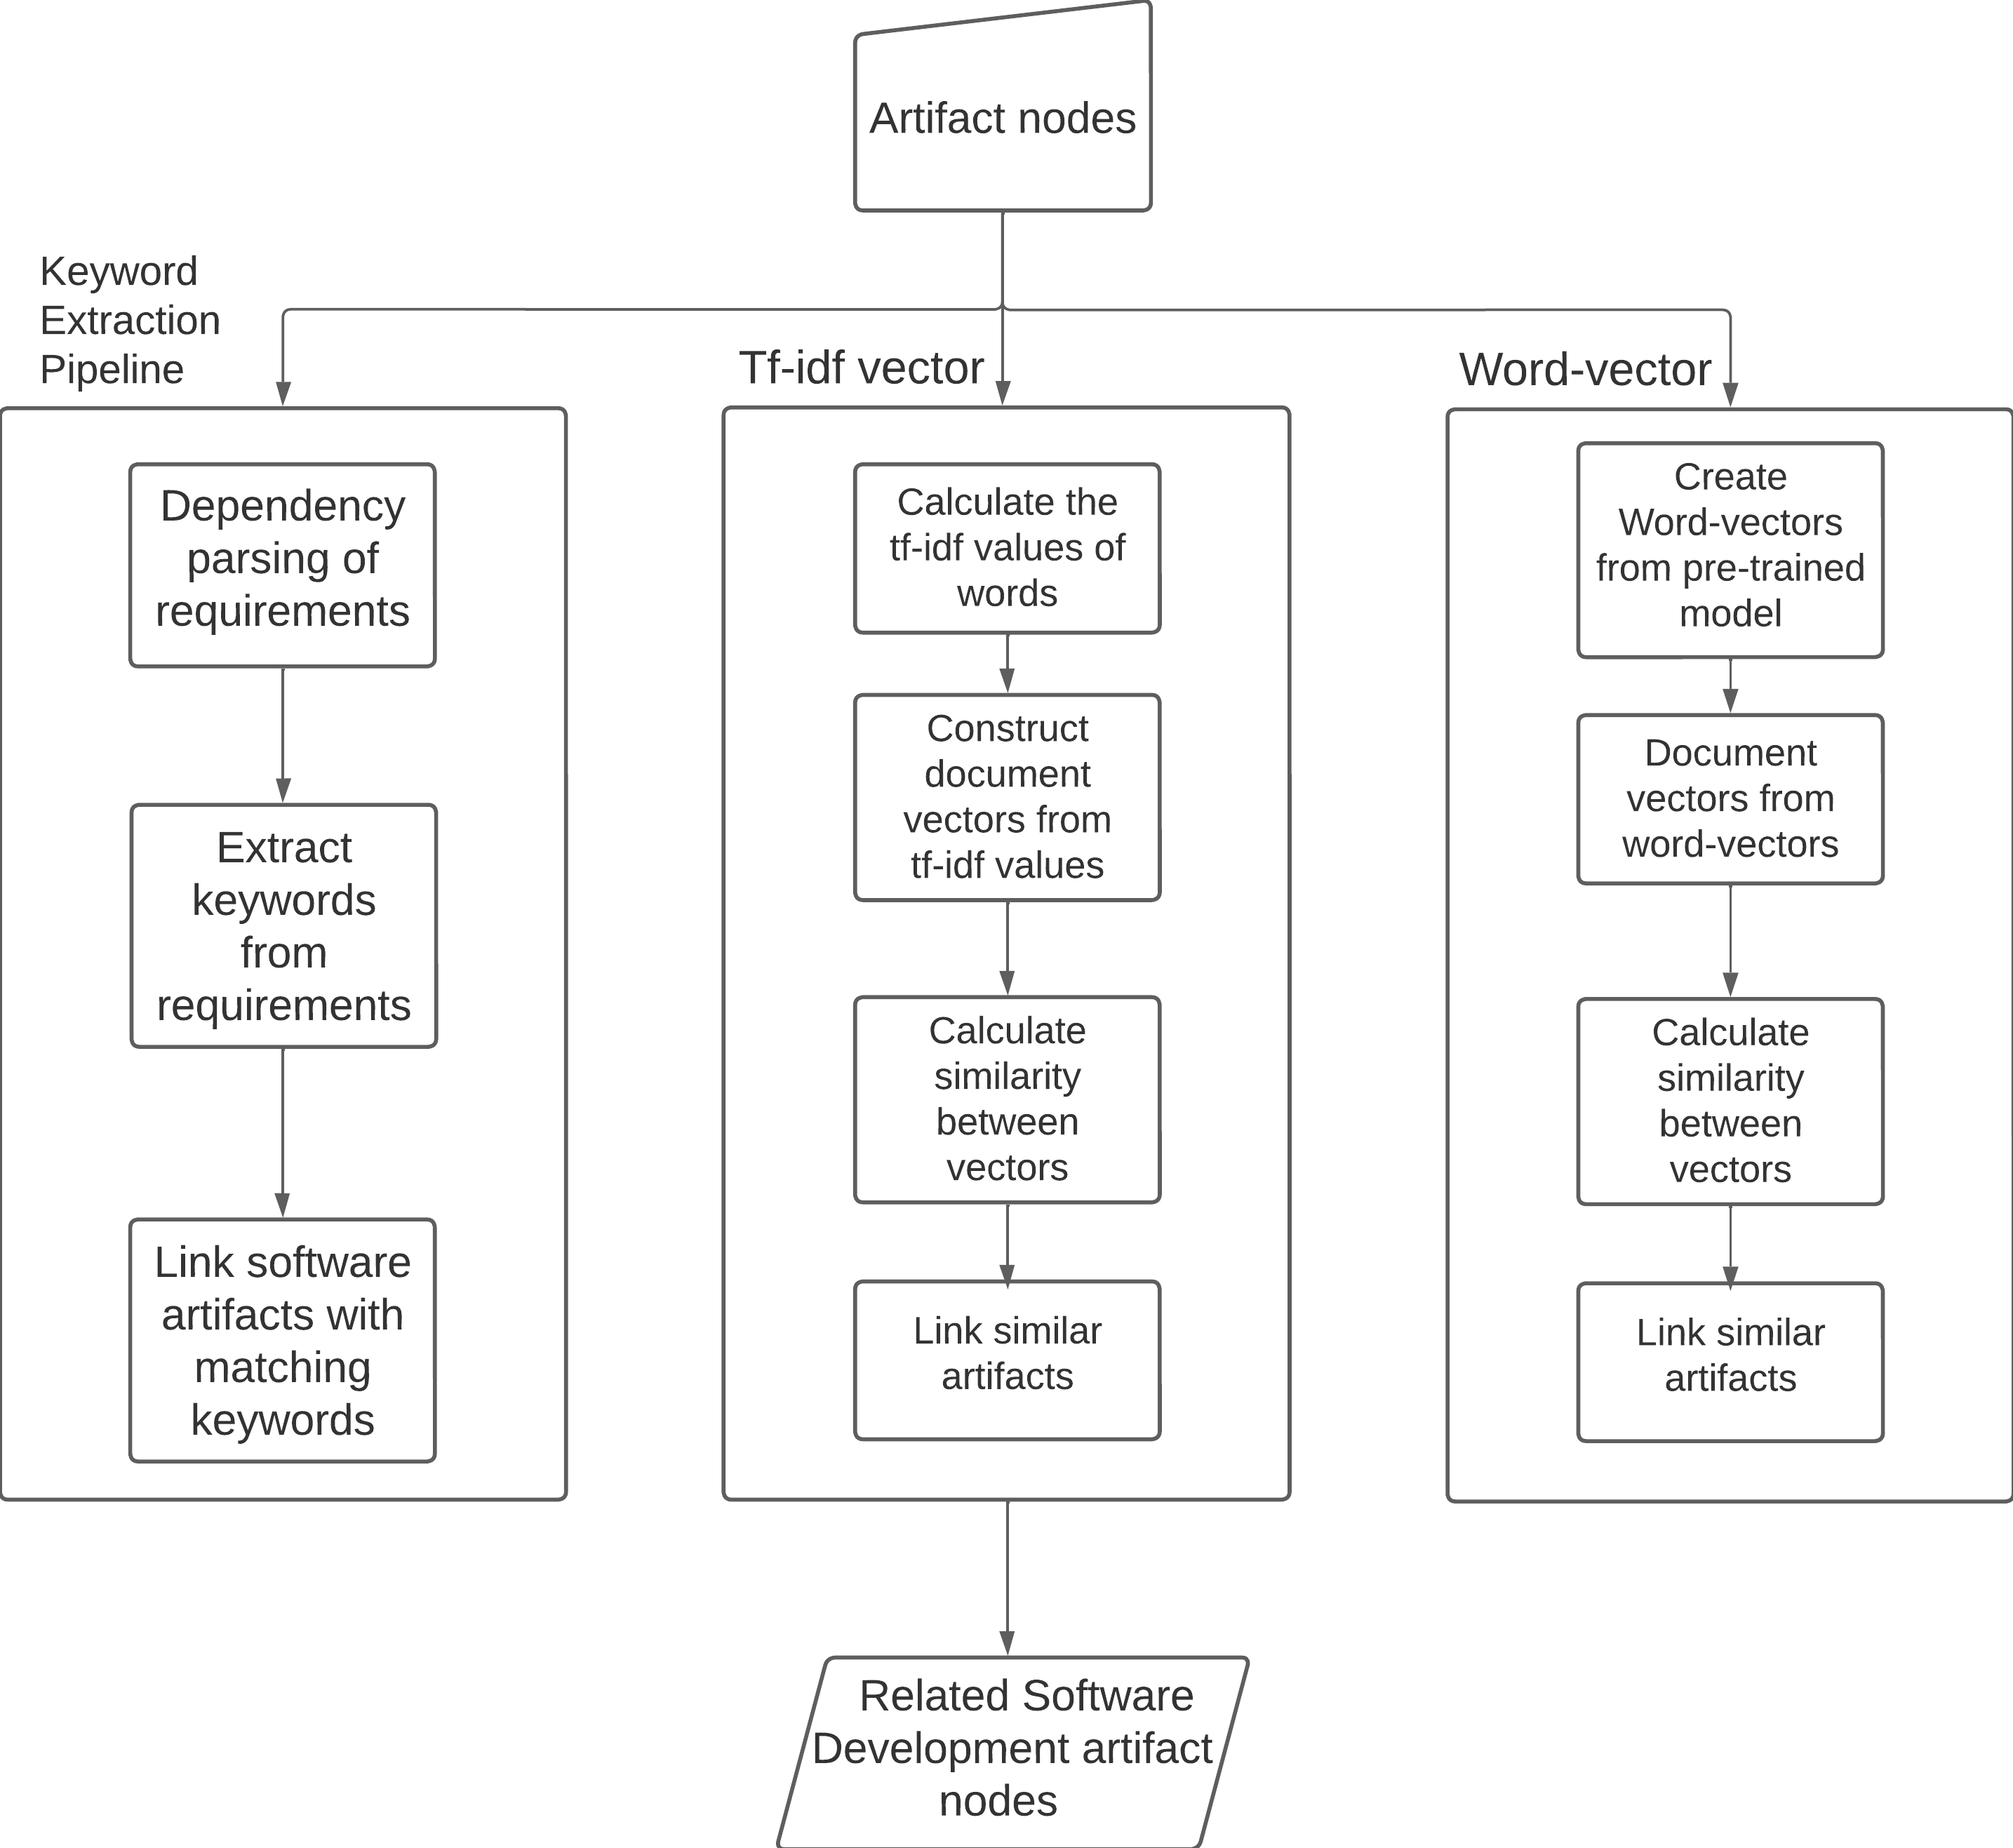
\includegraphics[width=0.9\linewidth]{figs/tracemethods.png}
      %   \caption{Control flow of the trace methods.}
      %   \label{fig:trace-methods}
      % \end{figure}

      \paragraph{Keyword Matching}

      \begin{figure}[htb]
        \centering
        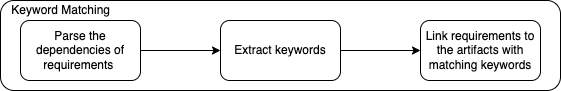
\includegraphics[width=0.99\linewidth]{figs/keywordmatching.png}
        \caption{Steps of trace link extraction based on keyword matching}
        \label{fig:keymatch}
      \end{figure}

      \paragraph{TF-IDF Vectors} We first build a corpus consisting of all words in the requirements and the software development artifacts. We remove the stop words from this corpus. We calculate the TF-IDF values and construct a TF-IDF vector for each requirement and artifact. We then link the requirements with artifacts that have a similarity score more than a threshold. In Sec.~\ref{sec:eval} we experiment with this threshold. Fig.~\ref{fig:tfidfvec} presents the steps for this method.



      \begin{figure}[htb]
        \centering
        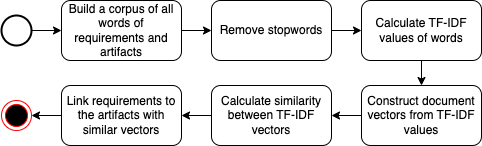
\includegraphics[width=0.99\linewidth]{figs/tfidfvector2.png}
        \caption{Steps of trace link extraction based on TF-IDF vectors}
        \label{fig:tfidfvec}
      \end{figure}

      \paragraph{Word Vectors}
       \begin{figure}[htb]
        \centering
        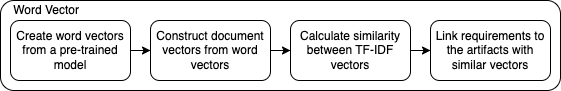
\includegraphics[width=0.99\linewidth]{figs/wordvector.png}
        \caption{Steps of trace link extraction based on word vectors}
        \label{fig:wordvec}
      \end{figure}







      %In the subsequent step, the file containing the information about SDAs and RDS are parsed to create graph nodes. At the completion of this operation, there are nodes representing each requirement and each SDA. The properties of the artifacts are stored as a property of the graph nodes. Later on, these nodes are saved into the graph database.

%Furthermore, the trace links for each requirement statement are identified. The tool has three different methods implemented for trace link recovery as displayed in Figure \ref{fig:trace-methods}. The first method involves a keyword extraction, where the significant keywords from requirement specification are extracted using a custom pipeline that utilizes \textit{dependency parsing}. These keywords serve as the basis for identifying trace links between SDAs and requirements. Keyword-matching is performed on the textual data of each SDA, to capture artifacts that include the keyword as a candidate trace. The second method utilizes the TF-IDF (Term Frequency-Inverse Document Frequency) algorithm, which creates a vector for each artifact, based on the importance of the terms in their textual data. By comparing the TF-IDF vectors, the potential trace links are identified. The third method acquires word embeddings for each artifact text using a pre-trained model, creating a document vector by averaging the word embeddings, and compares these vectors to identify traces, similar to the TF-IDF vector method.

%After the identification of the trace links, the graph database is utilized to store the trace links, along with requirements and SDAs. The use of a graph database offers a scalable solution and facilitates easy retrieval of traceability data through queries. More importantly, the graphical structure of the software artifacts and the requirements provides a comprehensive visualization of the trace links.

%Additionally, an interactive dashboard that visualizes the statistical information about the project and the requirements is developed. The dashboard includes various reports suitable for each kind of insight displayed, and facilitates a deeper understanding of the status and the complexity of the requirements, and provides information about the effort given to requirements during their lifetime.



\subsection{Heuristics}
\label{sec:heuristics}

\textbf{1 - Keyword Extraction}

To implement the keyword extraction method, a heuristic approach is taken, that includes several steps to extract the most relevant keywords from requirement statements. The steps of the process are as following:

\begin{figure*}
    \centering
    
\includegraphics[width=1\linewidth]{figs/displacy.png}
    \caption{Dependency tree for an example requirement statement.}
    \label{fig:deptree}
\end{figure*}

\begin{itemize}
    \item Tokenization and Part-of-Speech(POS) Tagging:
        \begin{itemize}
            \item Part-of-speech(POS) tagging is a process to assign a grammatical tag to each word to specify its syntactic role within a sentence. In this step, each word of the requirement statement is tokenized and the POS tagging is applied.
            \item By this process, each word of the requirement statement is categorized as nouns, verbs, adverbs, adjectives, etc.
        \end{itemize}


    \item Selecting Nouns and Verbs:
        \begin{itemize}
            \item Tokens that have \textit{noun} or \textit{verb} tag are extracted for further processing.
        \end{itemize}
    \item Dependency Parsing:
        \begin{itemize}
            \item Dependency parsing is the process of analyzing the dependency between the words of a sentence to discover the grammatical structure. In this step, a Dependency Parsing Tree of the requirement specification, which consists of dependency links is built.
            \item These links indicate the syntactic relationship between the words of a text.
            \item Figure \ref{fig:deptree} shows the POS tagging and the dependency tree of an example requirement statement. All of the words have grammatical categorization and syntactic dependency links in a tree structure.
        \end{itemize}

    \item Selecting Noun-Object and Verb-Object pairs:
        \begin{itemize}
            \item The dependency links of nouns and verbs created in previous steps are analyzed to capture direct objects that are linked to nouns/verbs.
            \item Nouns, verbs, and their corresponding objects are stored as "keywords" with labels \textit{noun-object} or \textit{verb-object}, based on the token tag.
        \end{itemize}
    \item Selecting Prepositions and Conjunctions:
        \begin{itemize}
            \item There are indirect objects linked to nouns and verbs using prepositions(e.g. on, at, it) and conjunctions(e.g. and, or). Further analysis is applied to noun and verb tokens to capture indirect objects and build phrases.
        \end{itemize}
    \item Removal of English Stopwords:
        \begin{itemize}
            \item English stopwords, such as articles, pronouns, and common conjunctions, are removed from the tokens.
            \item This process helps to reduce noise that could arise when keyword matching is applied to software development artifacts.
        \end{itemize}
    \item Optional: Removal of Project Specific Words from Requirement Specification Documents
        \begin{itemize}
            \item Words that are frequently used in the SDAs and requirement statements, which usually are not considered as english stopwords, are also removed.
            \item However, this step is considered optional and user is expected to provide such words.
        \end{itemize}
\end{itemize}

By employing this approach, the keyword extraction method effectively captures the significant keywords from requirement specifications and prepares a base for identifying trace links. Figure \ref{fig:keywords} shows the results of the method on an example requirement specification with the keywords extracted with their labels.

\begin{figure}[htb]
    \centering
    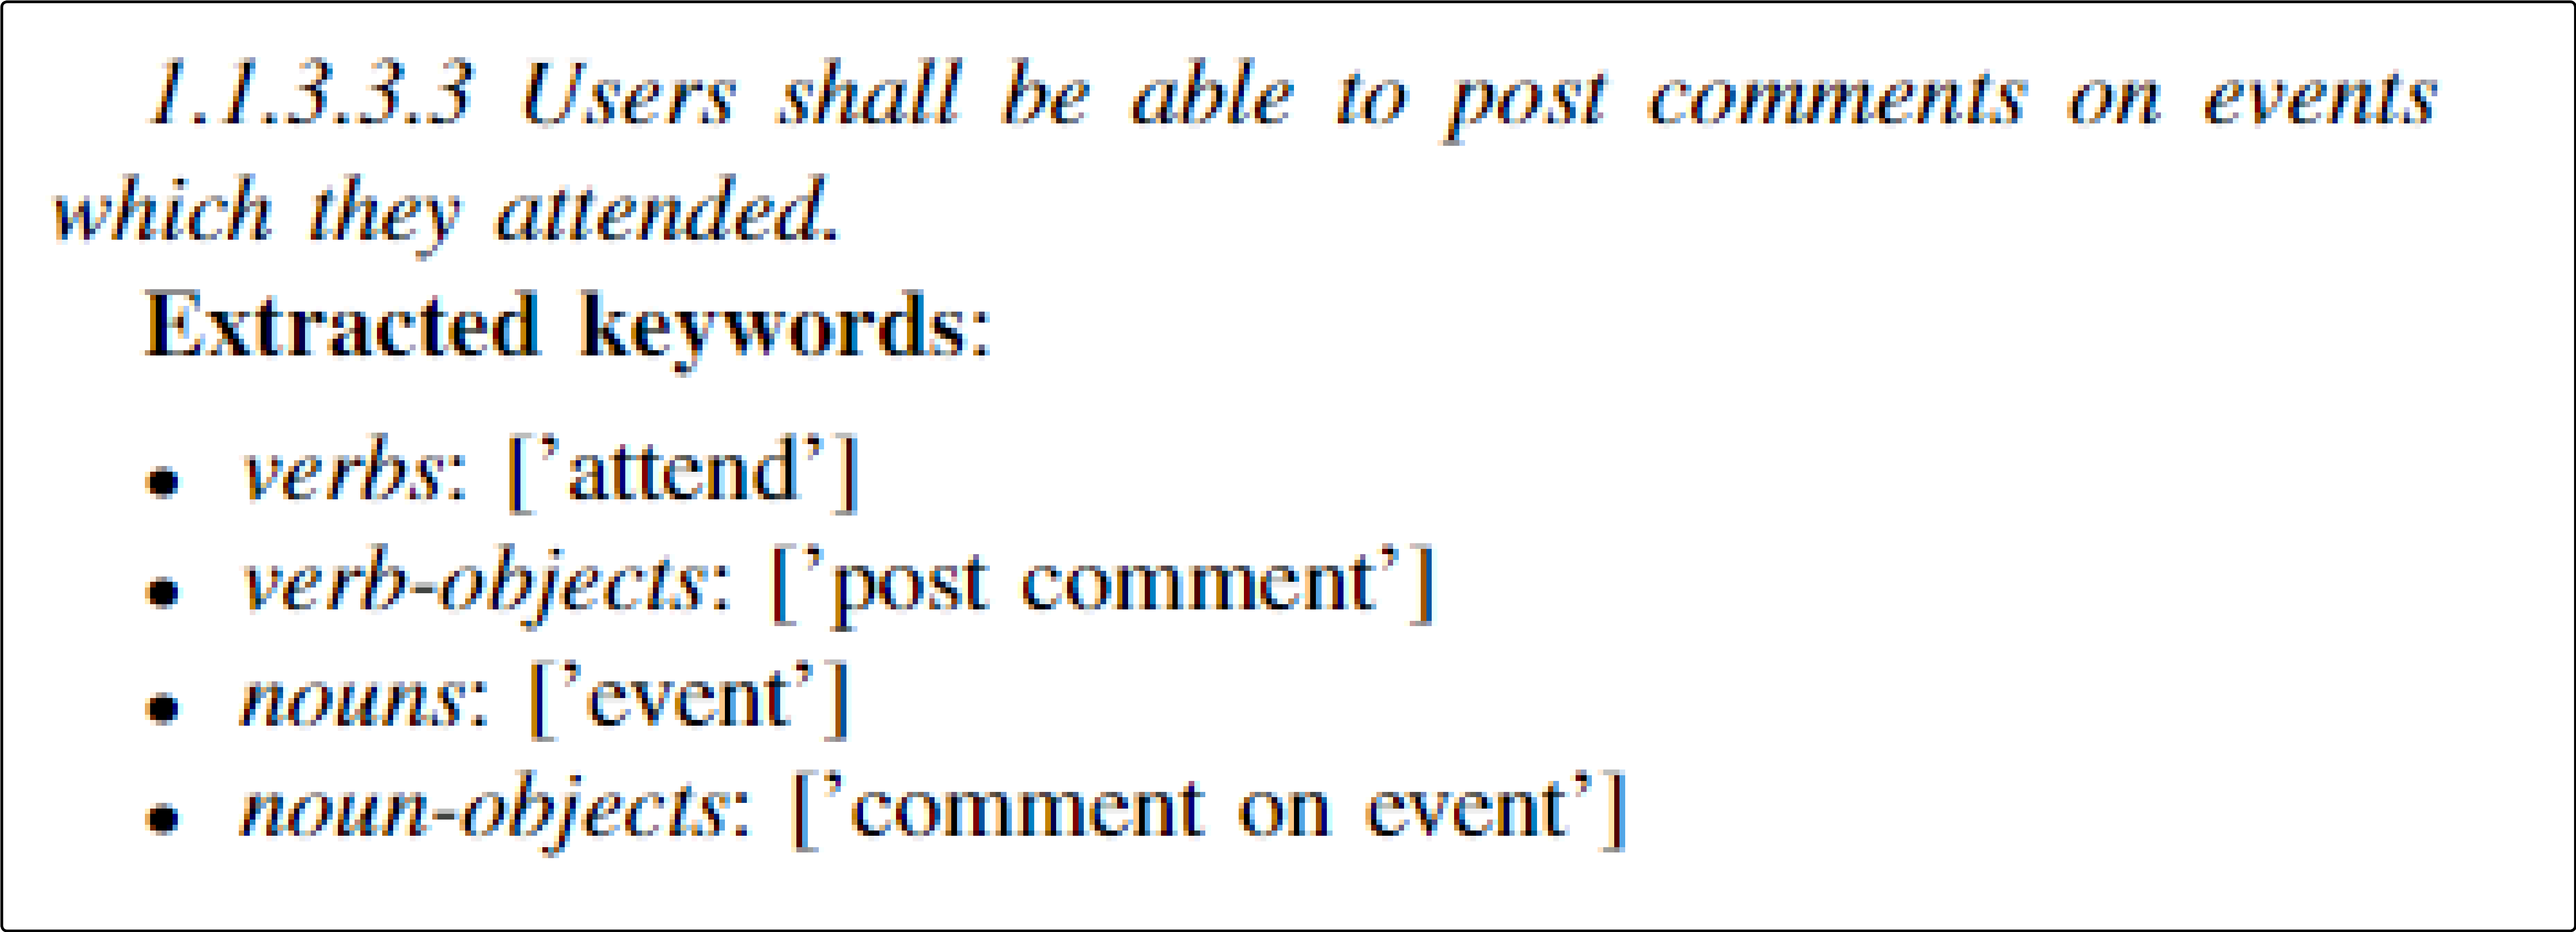
\includegraphics[width=1\linewidth]{figs/keywords.png}
    \caption{Results of keyword extraction on an example requirement specification.}
    \label{fig:keywords}
\end{figure}

The last step of the method is to perform keyword matching using regex statements among the textual properties of SDA(title, description, comments, etc.), and record the artifacts that have a match with at least one keyword as trace links.\\

% Initially, part of speech(PoS) tagging and dependency parsing is applied to the requirement statement(RS). This process reveals the grammatical tags of each word and their relation with each other. Then, the verbs and nouns of the RS are inspected.
% \begin{itemize}
%     \item Verbs and their related objects extracted as verb-object keywords.
%     \item Nouns and their compounds extracted as noun-phrase keywords.
%     \item Extra verb-object pairs extracted by inspecting conjunction links. In structures like \textit{"verb - object1 and object2"}(i.e. update username and password) verb usually has a link to the object1 and objects have conjunction link in between. Verb-object2 is extracted with this process.
%     \item Raw verbs that does not have any of these relations extracted directly.
%     \item Raw nouns are extracted directly in any case.
% \end{itemize}

% Further, these keywords are searched among the SDAs using regular expression matching and the SDAs that have matching keywords are recorded as candidate traces. (Should i include regular expressions themselves here)

\textbf{2 - Vector based methods}\\

\textit{TF-IDF vectors}

To generate tf-idf vectors for each artifact(SDAs and requirements):

\begin{itemize}
    \item A corpus is established by words consisted in all SDAs and requirements, except the english stopwords.
    \item Tf-idf value of each word in the corpus is calculated. (Figure \ref{fig:tfidf})
    \item A vector for each artifact is created by the tf-idf values of words contained in their text.
\end{itemize}


\begin{figure}[htb]
    \centering
    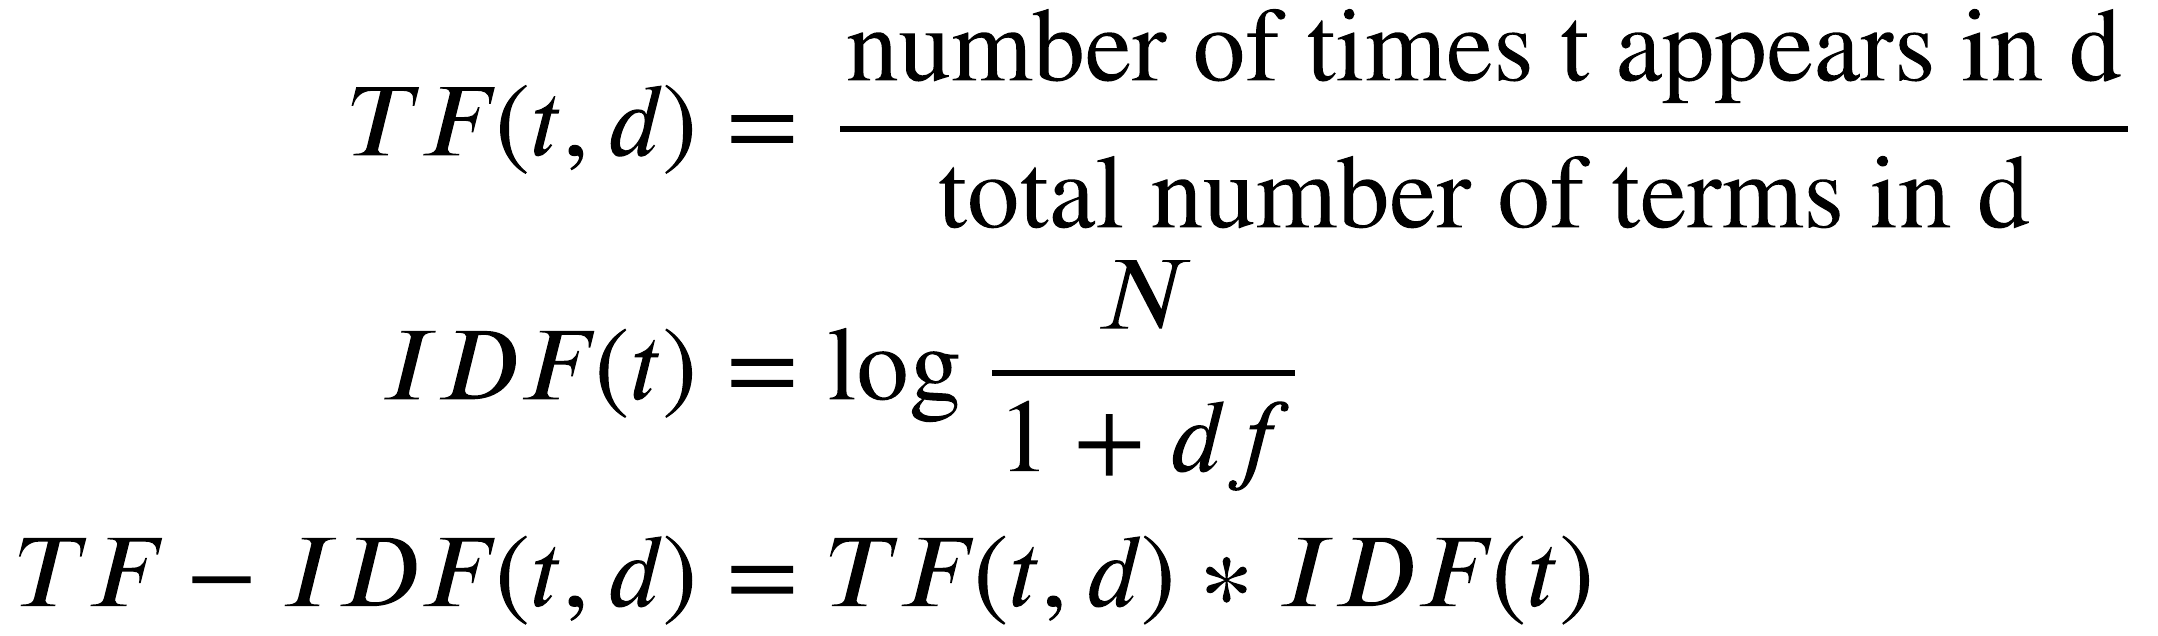
\includegraphics[width=0.75\linewidth]{figs/tfidf.png}
    \caption{TF-IDF equations.}
    \label{fig:tfidf}
\end{figure}


\textit{Word vectors}

To generate word vectors for each artifact:

\begin{itemize}
    \item A pre-trained word embeddings model is utilized.
    \item The word vector for each word within an artifact text is gathered from the model.
    \item A vector for each artifact is created by averaging the word vectors contained in their text.
\end{itemize}


The last step of the vector-based methods is to check the cosine similarity of the requirement vector with every other SDA. The artifacts that have similarity above the decided threshold are recorded as candidate traces.
%\textit{Heuristic 1 - Substring Match}. Our first heuristic depends on the substring matches that can be observed among noun phrases. This process can be briefly explained as clustering noun phrases with the subset of noun phrases that contain a particular noun phrase as a substring. For example, "item label" and "item label size" noun phrases will be clustered under the "item label" key because "item label size" denotes a property of "item label". By applying this heuristic, all of these noun phrases are clustered into a set and the shortest noun phrase will represent these noun phrases. This heuristic reduces the size of the initial set of noun phrases. The reduction in the size of the initial set of noun phrases also decreases the time and space complexity of further steps of processing.

%After applying the first heuristic, we manage to cluster some of the model labels. However, there are still independent model labels. Even though the models are generated by modeling experts, modelers with different backgrounds may use different words for the same concept. For example, "shipment options" and "shipping offers" will be matched as similar noun phrases because of the high level of relatedness between the two of the noun phrases. To increase coverage of the NLP pipeline, we benefit from BERT \cite{devlin2018bert} which is a state-of-the-art deep language model. Thus, glossary extraction from models is provided by measuring the similarity of different noun phrases to each other and detecting different noun phrases that refer to a similar meaning via pre-trained sentence embeddings.

%First, noun phrases are encoded using sentence transformers which are provided by Hugging Face\footnote{https://huggingface.co} and are designed to be used with a pre-trained model. There is a variety of pre-trained sentence embedding models available for sentence embedding. We choose \textit{paraphrase-mpnet-base-v2} due to its high performance on STSbenchmark test. This sentence encoding process yields vectors that have 768 dimensions for each noun phrase. To extract similar noun phrases, pairwise cosine similarities are calculated between each noun phrase, and the symmetrical similarity matrix is obtained.




%\begin{algorithm}[htp]
%\SetAlgoLined
%\SetKwInOut{input}{Input}
%\SetKwInOut{output}{Output}
%\input{parent term P and term T}
%\output{parent term}
%parent = P\;
%term\_string = T + parent\;
%keywords = extracted keyword and probability pairs from term\_string using KEYBERT\\
%\uIf{length of keywords $>$ 1}{
%set most probable keyword as parent\\
%}
%\textbf{return} parent\;
% \caption{Heuristic 3}
%\end{algorithm}

%\textit{Heuristic 3 - Keyword Extraction}. Keyword extraction methods are mostly used for extracting the most representative n-grams from the texts. In this heuristic, lemmatized versions of both key and value are collected for each pair and concatenated into a single string. (Line 2) KeyBERT is tuned to extract unigrams from that concatenated string. (Line 3) If there exists a smaller common unit of representation for a key-value pair, both key and value are clustered under that new representation. (Lines 4 - 5)

%After applying these steps, all noun phrases extracted from the models are stored in a dictionary for reporting and visualized using an undirected graph for better understanding. Fig \ref{fig:graph} shows a sample representation extracted glossaries. Blue vertices denote matching model labels with concepts and red vertices (self-links) denote the mismatched model labels.

%\begin{figure}[htp]
%    \centering
%    \includegraphics[width=0.9\linewidth]{figs/graph.png}
%    \caption{Sample graph representation of extracted terms}
%    \label{fig:graph}
%\end{figure}

\subsection{Trace Graph}
\label{sec:tgraph}

The construction of the trace graph requires parsing the requirement specifications and the software development artifacts(Issues, PRs, Commits) to create graph nodes, and executing several methods to identify trace links between them. The graph nodes have various properties associated with them to store detailed information about the artifact that they represent.
Table \ref{tab:artifactfeatures} displays the properties of the different kinds of graph nodes encapsulates.


% \begin{table}[htb]
% \begin{adjustbox}{width=1\linewidth}
% \begin{tabular}{|l|c|c|c|c|c|c|}
%         \hline
%  &                & Requirement & Issue & PR  & Commit &  \\\hline\hline
%  & Id             &  \checkmark & \checkmark & \checkmark & \checkmark    &  \\\hline
%  & Title          & -           & \checkmark   & \checkmark     &   -     &  \\\hline
%  & Description    & \checkmark         & \checkmark   & \checkmark     & -       &  \\\hline
%  & URL            & -           & \checkmark   & \checkmark     &  \checkmark       &  \\\hline
%   & Number           & \checkmark   & \checkmark  &  \checkmark  & \checkmark  &  \\\hline
%    & State           &  -           & \checkmark       &  \checkmark    & -     &  \\\hline
%  & CreationDate   & -           & \checkmark   & \checkmark & -      &  \\\hline
%  & CompletionDate & -           & \checkmark   & \checkmark     & \checkmark    &  \\\hline
% & Message        & -           & -   & - & \checkmark    &  \\\hline
%  &  CommentCount         &  -           &  \checkmark      & \checkmark     &       - &  \\\hline
%   &  CommentList         & -            & \checkmark       & \checkmark     &      -  &  \\\hline
%    &   Parent         &   \checkmark           &  -     &  -   &  -      &  \\\hline
%     &   Oid          &    -         &  -     &   -  &  \checkmark       &  \\\hline
%      &  Text       &  \checkmark            &  \checkmark      &  \checkmark    & \checkmark        &  \\\hline

% \end{tabular}
% \end{adjustbox}
%         \caption{\label{tab:artifactfeatures} The features of the artifacts utilized in identifying trace linking.}
%       \end{table}



The textual properties of the nodes are required for the vector-based and keyword extraction trace identification methods to operate. In addition, the properties enable the observation of the creation/closure times and the status of the artifacts. Moreover, it is possible to access  the GitHub page that they are acquired from with URL property. Overall, these properties provide valuable traceability data, which serve as a foundation for an interactive dashboard that provides project management and requirement lifecycle analysis.

 Along with the artifact nodes, two types of relationships are in use to show the relationship between the artifacts, namely \textit{tracesTo} and \textit{relatedCommit}. The \textit{tracesTo} relationship represents an identified trace link and could be present between a requirement node and a software development artifact node. On the other hand, \textit{relatedCommit} relationship detonates a Commit associated with a PR, hence it could be present between a PR node and a Commit node.

To store the highly interlinked software artifacts the graph database Neo4j was chosen.
In addition to its ease of use, the query interface with effective visualizations was beneficial during the analysis phase of this work.

Fig. \ref{fig:rawtracegraph} illustrates a segment of the trace graph obtained from the Neo4j graph database for a specific requirement and displays the associated trace links and related commits.

\begin{figure}[htb]
    \centering
    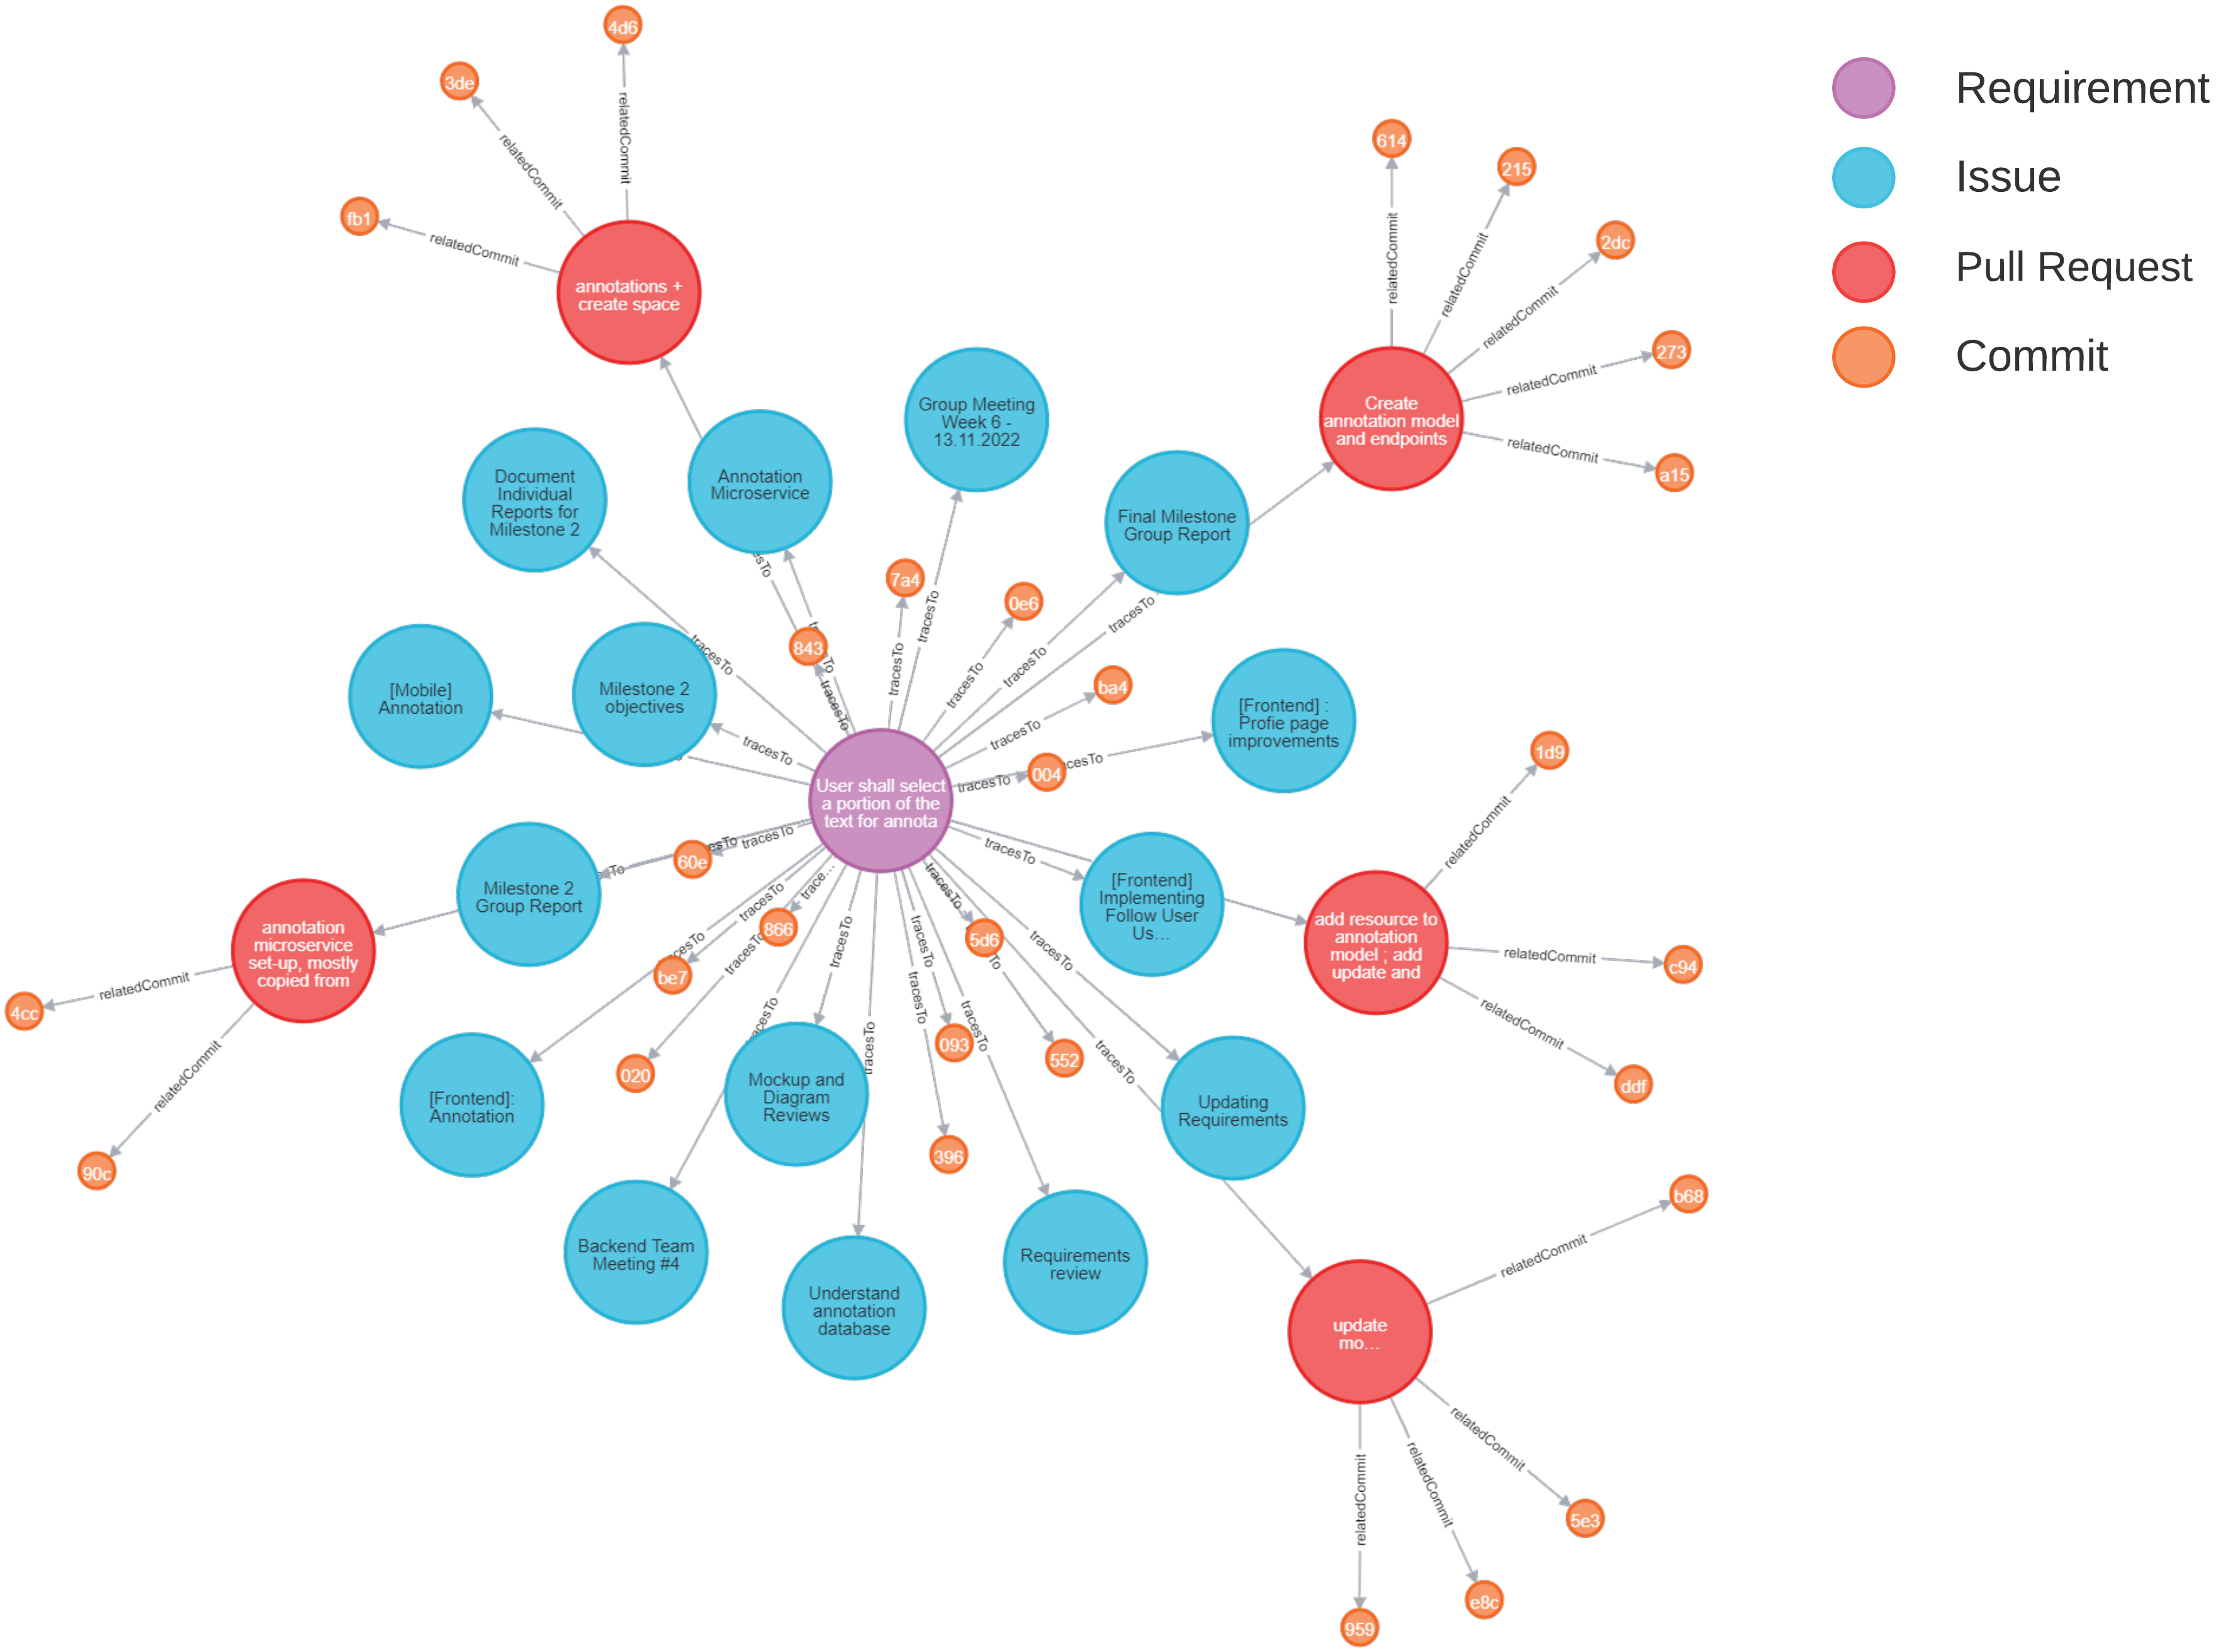
\includegraphics[width=1\linewidth]{figs/rawTraceGraph.png}
    \caption{A segment of the trace graph.}
    \label{fig:rawtracegraph}
\end{figure}

The trace graph serves as an effective visualization of the software development artifacts (SDA) that are traced to the requirement. Moreover, it has the potential to display the lifetime of the requirement when the traced SDA are organized chronologically.
In Fig. \ref{fig:tracegraph} the related SDA are arranged along a time axis based on their \textit{creationDate} property in order to represent notable information about the stages of implementation. For example, it is observed in the figure that the first Pull Request related to the requirement was created in week 8, while the issues concerning the planning of the requirement were created in the early stages of the development.


\begin{figure}[htb]
    \centering
    
\includegraphics[width=1\linewidth]{figs/traceGraph.png}
    \caption{Trace graph on a time axis.}
    \label{fig:tracegraph}
\end{figure}

% - The requirement to be examined is the root.
% - The requirement is connected to its related SDAs with \textit{tracesTo} links.
% - Pull request nodes have related commit nodes connected with \textit{relatedCommit} link.

% Who looks at trace?\\
% Trace graph can help a project manager or a developer
% Why?\\
% What can be found?


% A project manager looking at the trace graph can identify:

% \begin{itemize}
%     \item The planning phase of this requirement goes back to week 1
%     \item The implementation of this feature started at week 8
%     \item This requirement took around 13 weeks of work??
%     \item ...
% \end{itemize}

% \pagebreak

% Or in the case of a problem or a bug related to annotation, for example, a developer can view the trace of the requirement about annotation, localizing the search for the problem. Lets say the problem is about updating annotations. Looking at the trace graph, an educated guess can be made, with the information about the problem, to look at a specific pull request. For example, in our case user can view \textit{"Create annotation model"} and \textit{"... add update and delete annotation endpoints..."} nodes. Both nodes can be further observed by using the url property, reaching the github page and examining the code related to them.



\subsection{Dashboard}
\label{sec:dboard}


In order to reinforce the visualization of traceability data, our research includes the development of an interactive dashboard, which offers various reports that display statistical insights. Each of these reports was carefully selected to effectively visualize the corresponding data, hence they have user-friendly designs for enhanced comprehension. Moreover, many of these reports are interactive and they allow users to trace the specific requirements, thereby enabling a more customized exploration of the traceability information.
The dashboard was implemented using Neodash technology, to provide full integrity with the traceability graph that is stored in the Neo4j database.

The first report featured in Fig. \ref{fig:barcharts} is a stacked bar chart showing the number of created Issues(in green) and PRs(in brown). It could be observed that the highest number of created artifacts were in week 3 and week 7. The next report is another stacked bar chart that represents the number of artifacts opened and closed per week. Both of these charts are providing information about the status of development in the project lifetime and they help to identify periods of high or low development intensity and let users observe the assessment of the overall project dynamics.

The dashboard also provides static data regarding the number of open/closed issues, the number of open/merged PRs, and the average number of trace links per requirement. These statistics serve as a snapshot of the current state of the project.

\begin{figure}[htb]
    \centering
    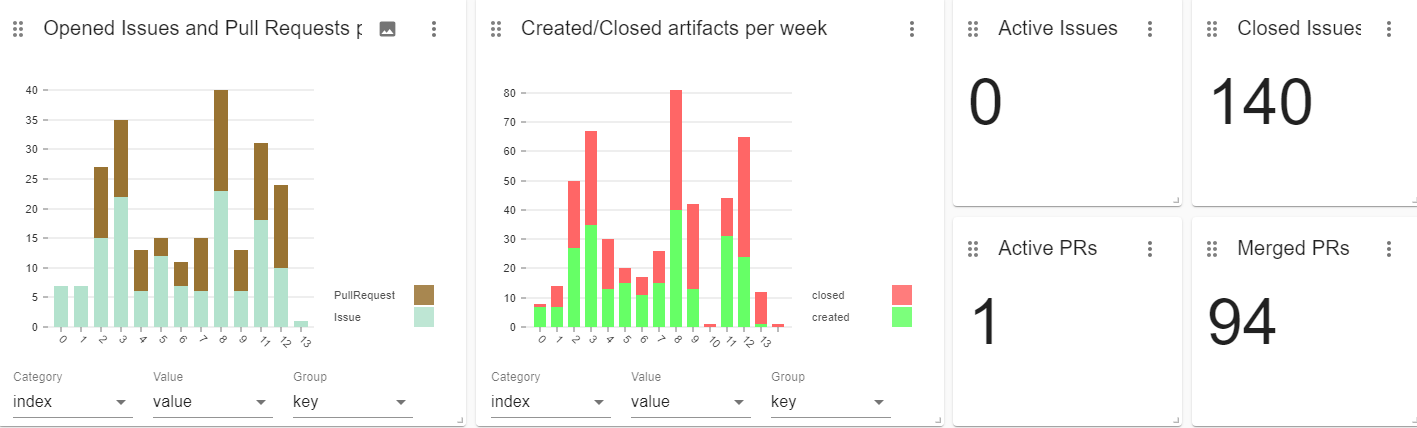
\includegraphics[width=1\linewidth]{figs/dashboard-barcharts.png}
    \caption{Bar charts and static data on dashboard.}
    \label{fig:barcharts}
\end{figure}

Fig. \ref{fig:linechart} continues with the line chart that illustrates the number of trace links for each requirement. By comparing the number of traces for each requirement, the report demonstrates the outliners, that could have relatively less or more traces. This comparison allows the users to observe the effort associated with each requirement since it displays the number of software development artifacts traced to them.

\begin{figure}[htb]
    \centering
    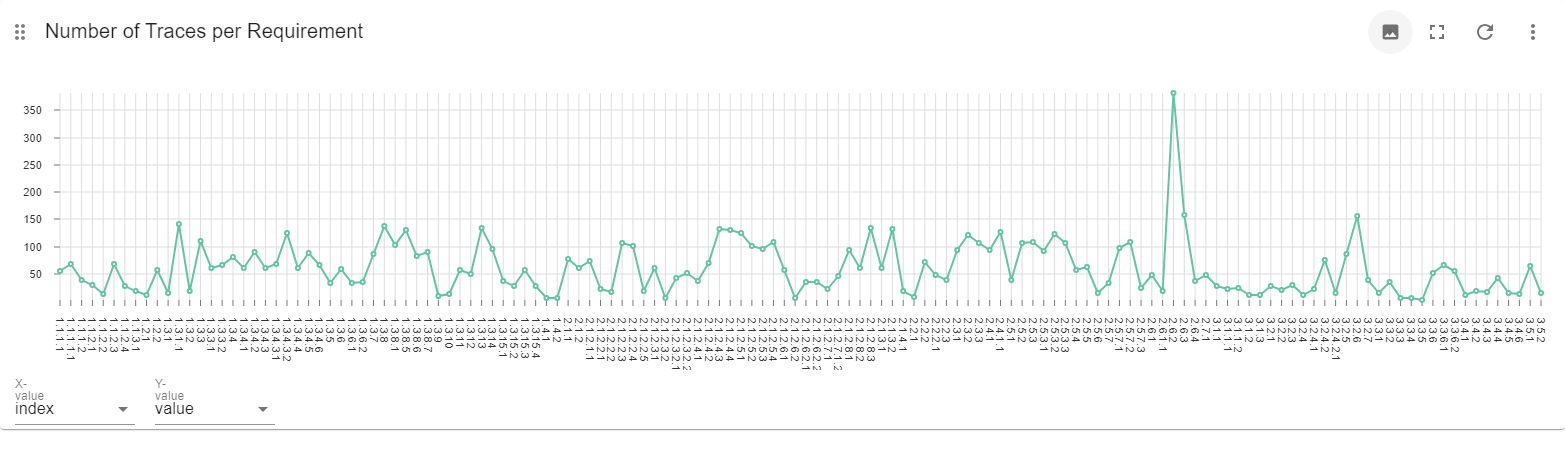
\includegraphics[width=1\linewidth]{figs/linechart.png}
    \caption{Line chart on dashboard.}
    \label{fig:linechart}
\end{figure}

Fig. \ref{fig:sankey} includes an example of the Sankey chart present in the dashboard that showcases the commonly traced artifacts between the chosen requirements while highlighting the strength of the trace links using the weight property. Thicker links represent a stronger relation from the requirement to the traced artifact. Thus, the chart represents the complementarity of the selected requirements.

\begin{figure}[htb]
    \centering
    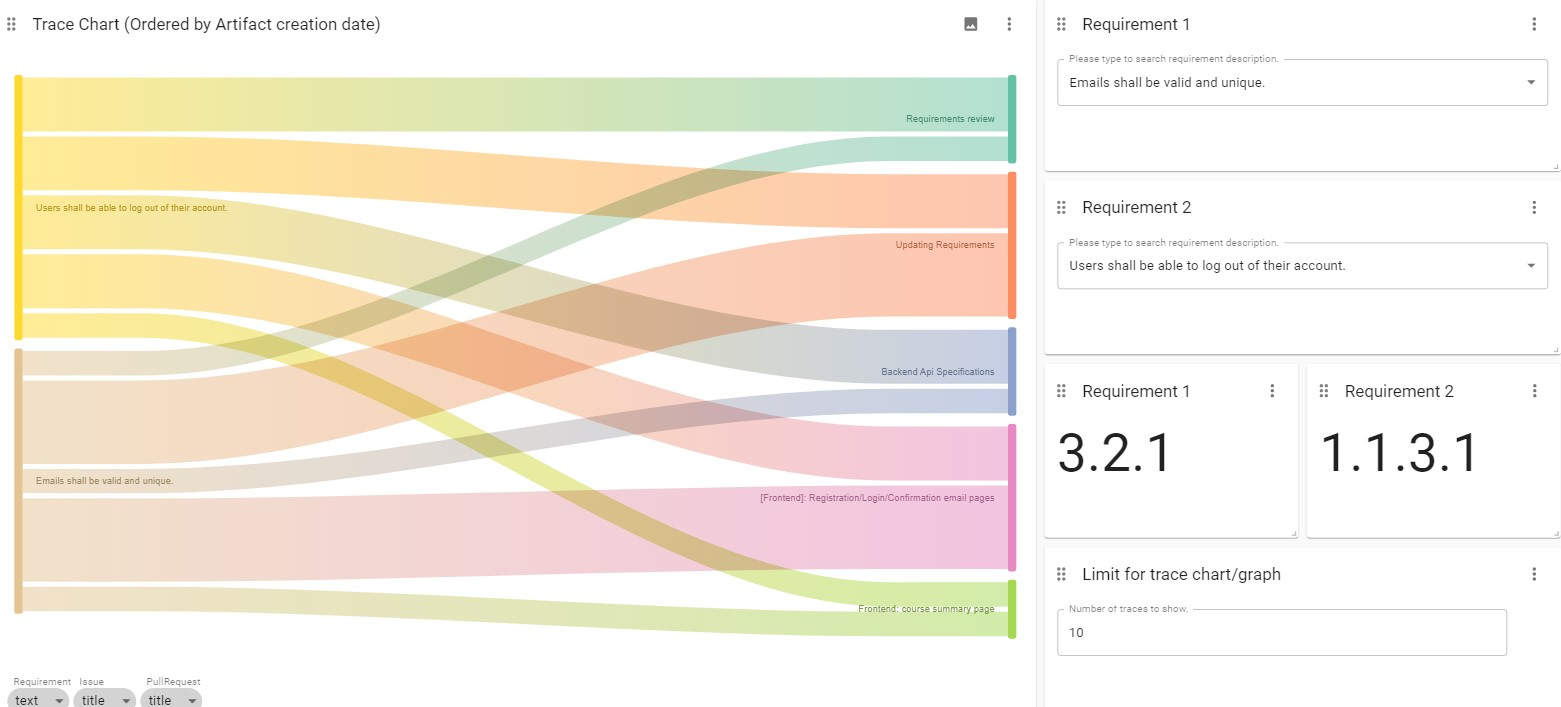
\includegraphics[width=1\linewidth]{figs/sankey.jpg}
    \caption{Sankey chart on dashboard.}
    \label{fig:sankey}
\end{figure}

As displayed in Fig. \ref{fig:perreq}, in addition to the generalized insights about the project status, various reports are implemented offering similar data for a specific requirement selected by the users. These include bar charts, similar to the earlier reports, tabular and graphical versions of the identified traces for the selected requirement. Overall, the current status and weekly effort given on a selected requirement are displayed in the last section of the dashboard.

\begin{figure}[htb]
    \centering
    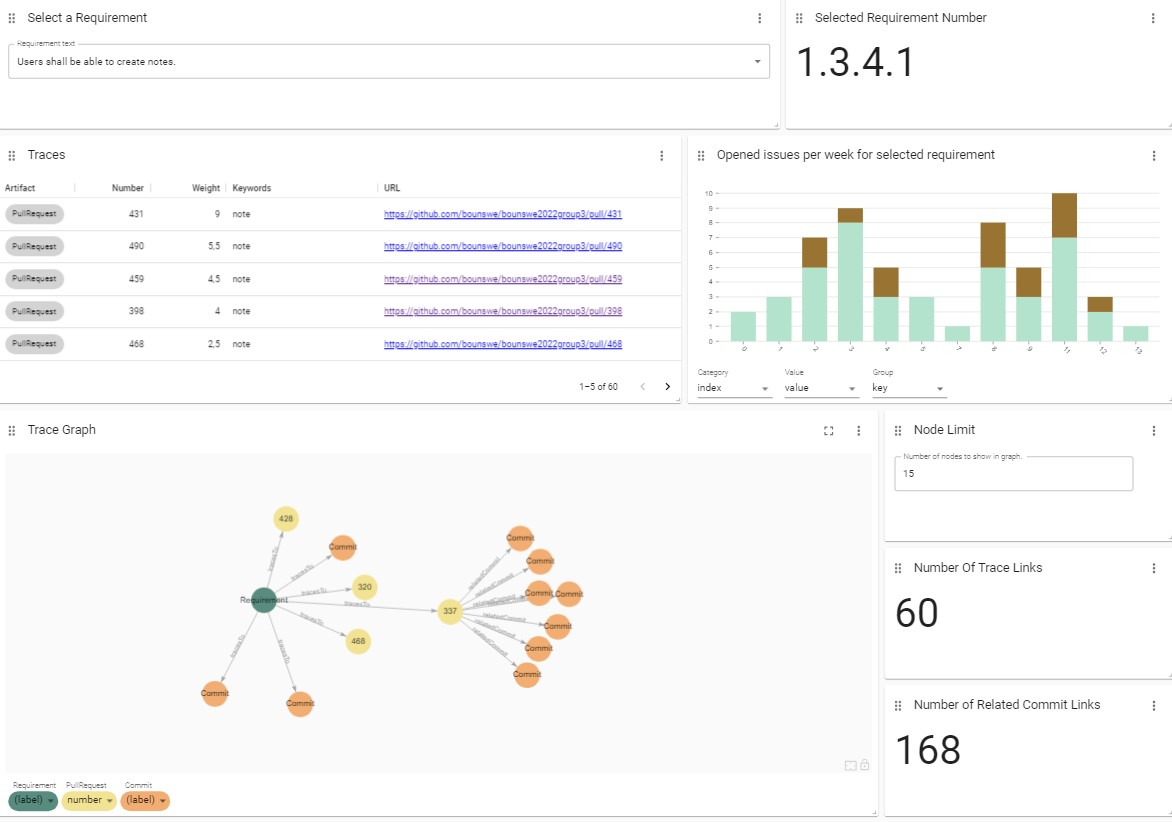
\includegraphics[width=1\linewidth]{figs/perreq.jpg}
    \caption{Insights for the selected requirement on dashboard.}
    \label{fig:perreq}
\end{figure}

%%% Local Variables:
%%% mode: latex
%%% TeX-master: "../main"
%%% End:
